
%----------------------------------------------------------------------------------------
%	SECTION 3
%----------------------------------------------------------------------------------------

\section{Hultin \& Lundquist Arkitekter, June 2017}

%\subsection{Architecture Placement at Hultin \& Lundquist Arkitekter in Malm\"o, Sweden}
During my second placement at Hultin \& Lundquist Arkitekter, I:
\begin{itemize}
	\item Produced window, door and kitchen schedules on AutoCAD.
	\item Was responsible for daylight calculations of a new-build during planning stage.
	\item Began a feasibility study on the construction of recycling sheds to five existing apartment buildings shortly before the end of my placement.
\end{itemize}

%How did I progress or what did I learn during this placement?
I had to be creative in clearly displaying the numbers and types of doors, kitchens and apartments in schedules.
I achieved this through the use of tables, as seen in Figure \ref{fig:schedules}.
I also improved my conditional formatting skills in spreadsheets during my work on daylight calculations.
%Practised my 2D AutoCAD skills again.
%Took measurements to double-check the accuracy of outdated drawings.
%Apart from these things which were somewhat stimulating, I found the tasks I was given a bit monotonous.

\begin{figure}[htbp]
	\centering
	\begin{subfigure}{.48\textwidth}
		\centering
		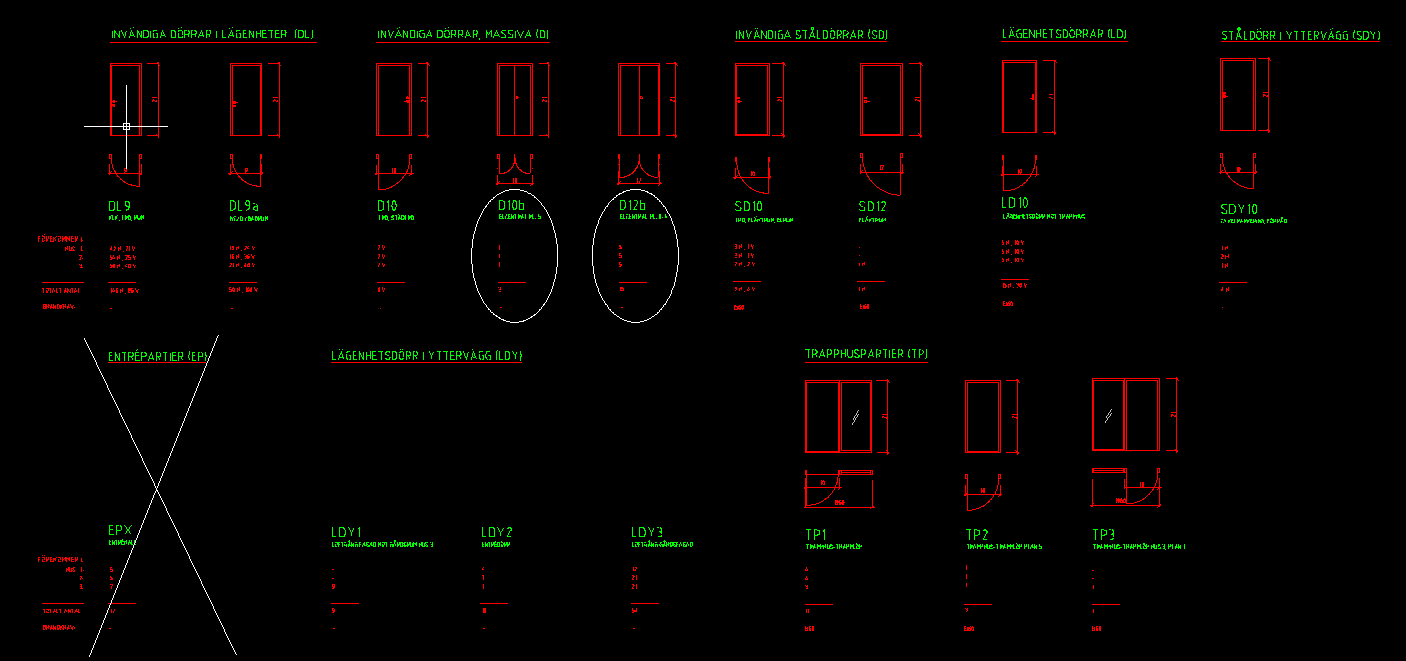
\includegraphics[height=4cm]{figures/door-schedule.png}
		%          \rule{\textwidth}{0.5pt} % use line???
		\caption{Door schedule}
		\label{fig:sched_doors}
	\end{subfigure}
	\begin{subfigure}{.48\textwidth}
		\centering
		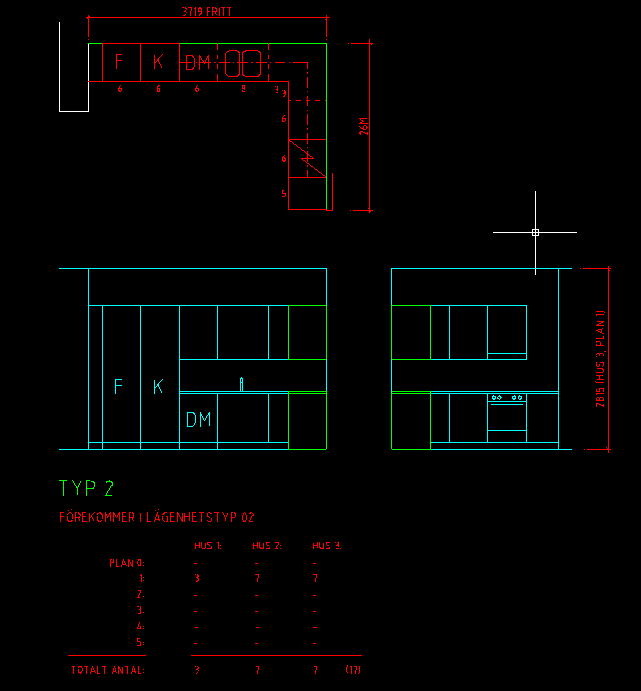
\includegraphics[height=4cm]{figures/kitchen-schedule.png}
		%          \rule{\textwidth}{0.5pt} % use line???
		\caption{One of the kitchen schedules}
		\label{fig:sched_kitchen}
	\end{subfigure}
	\rule{\textwidth}{0.5pt} % use line???
	\caption[Hultin \& Lundquist Arkitekter schedules.]{Screenshots of schedules done in AutoCAD at Hultin \& Lundquist Arkitekter.}
	\label{fig:schedules}
\end{figure}